\chapter{Chaos analysis of multiple oscillators}

\section{Two blocks}

The coupling between two oscillators is performed by connecting
the inverted voltage $-W_2$ of the second oscillator to the
first one and viceversa, as shown in Fig.
\ref{fig:breadboard implementation}. A chaotic behavior can be observed,
as can be seen in Fig. \ref{fig:2 blocks waveforms}.


\begin{figure}[H]
    \centering
    \begin{minipage}{.49\textwidth}
        \begin{subfigure}{\linewidth}
            \centering
            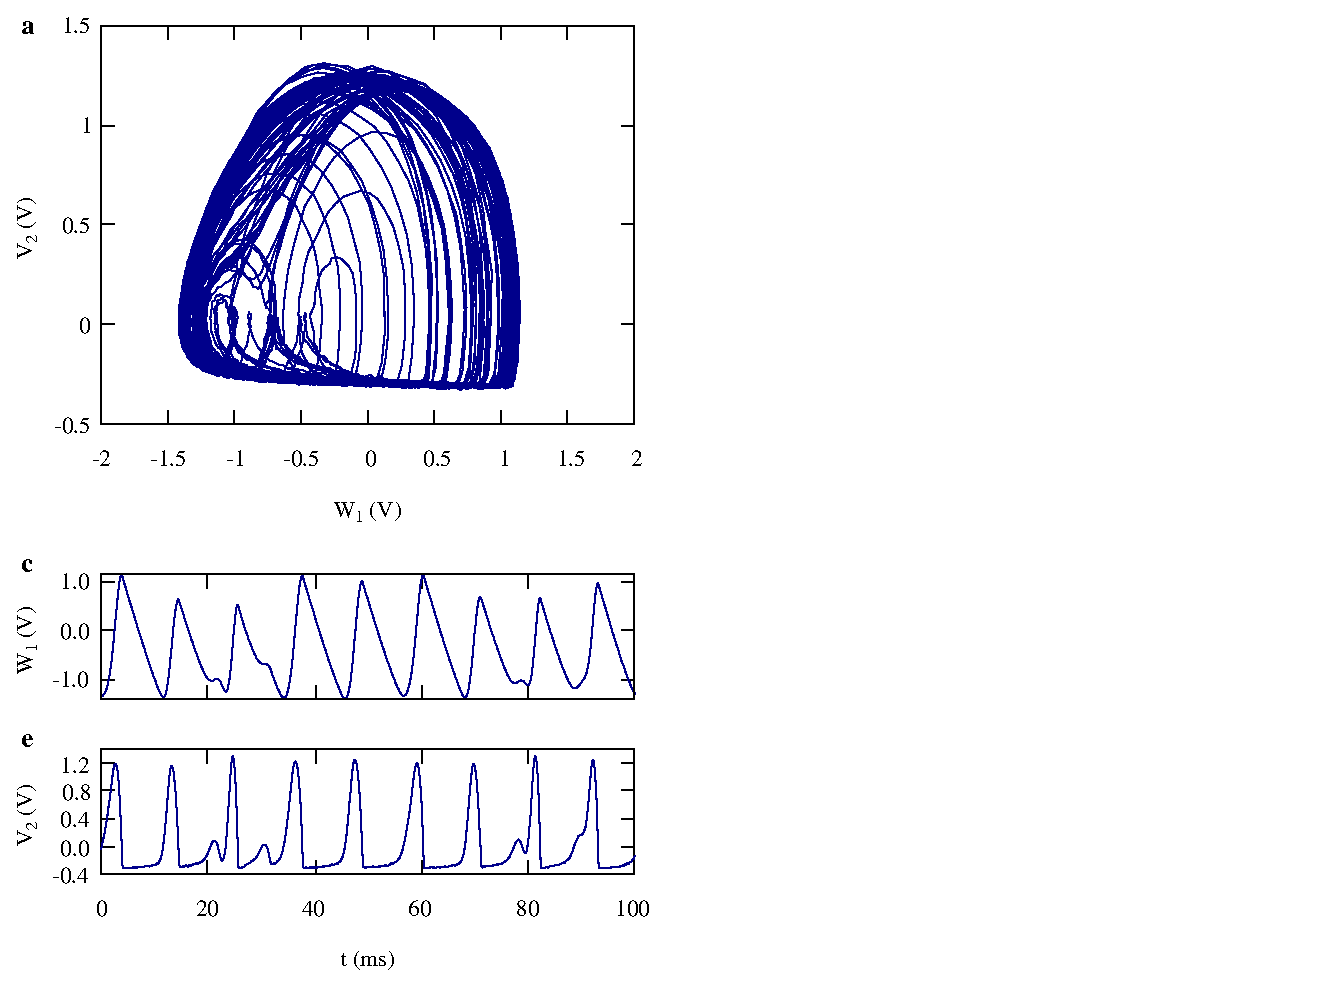
\includegraphics[width=\linewidth,trim={0cm 0 11cm 0},clip,center]
            {../2_blocks/4e4_points/plots/waveforms_1.pdf}
        \end{subfigure}
    \end{minipage}
    \begin{minipage}{.49\textwidth}
        \begin{subfigure}{\linewidth}
            \centering
            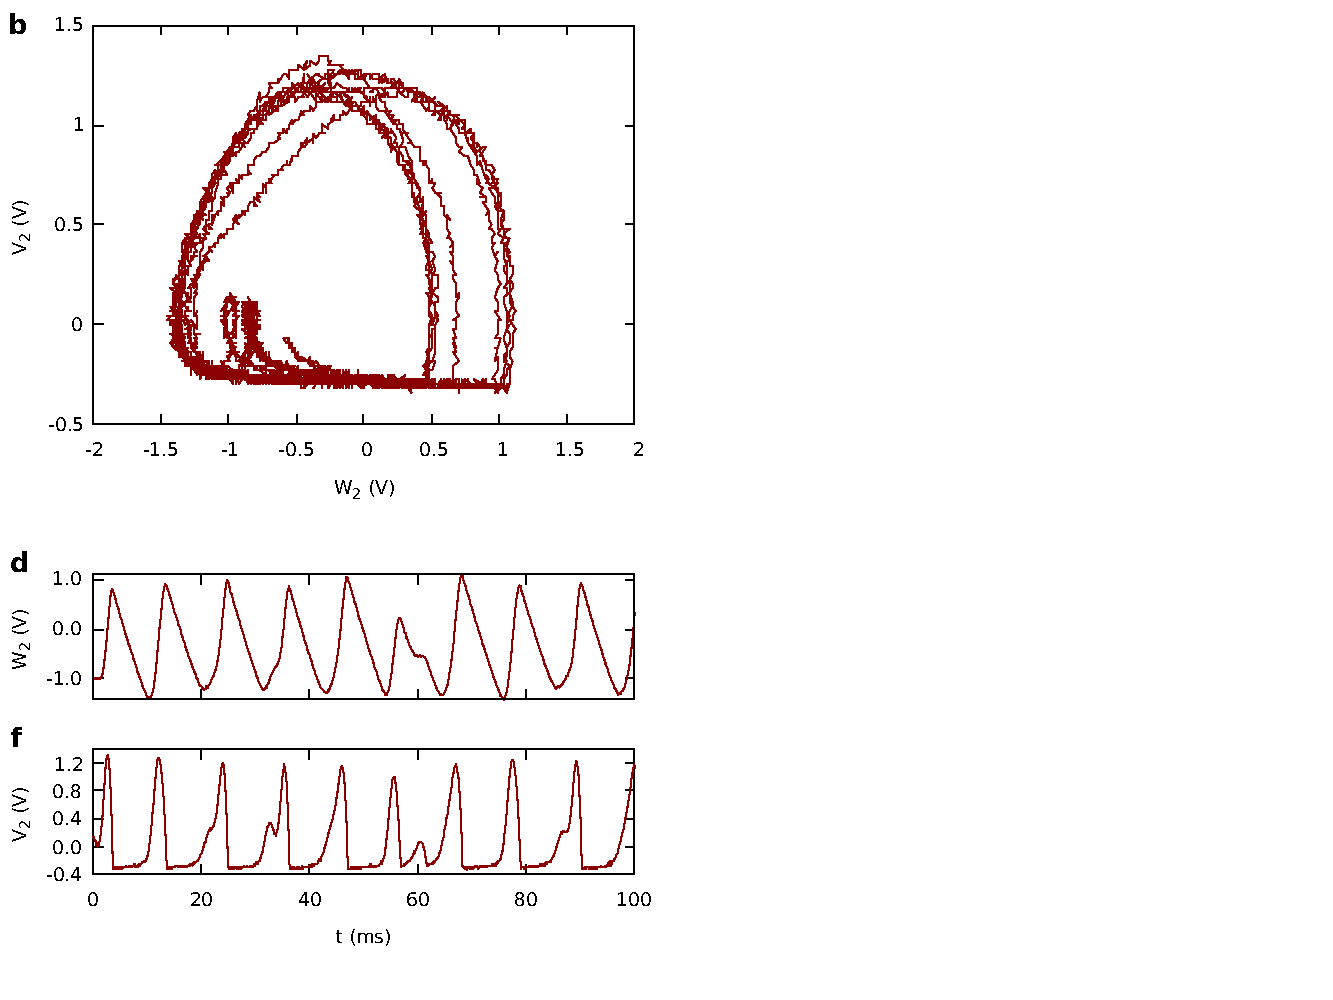
\includegraphics[width=\linewidth,trim={0cm 0 11cm 0},clip,center]
            {../2_blocks/4e4_points/plots/waveforms_2.pdf}
        \end{subfigure}
    \end{minipage}
    \caption{Chaotic behavior of two coupled blocks for
    $V_d=0.05$ V and for a total time of 100 ms. Phase portraits of $V_i$
    vs $W_i$ for the first (a) and second (b) block. Time series plots
    for $W_1$ (c), $V_1$ (e), $W_2$ (d) and $V_2$ (f).}
    \label{fig:2 blocks waveforms}
\end{figure}

In order to quantify the degree of chaos of this system, it is possible
to carry out an analysis

\begin{figure}[H]
    \centering
    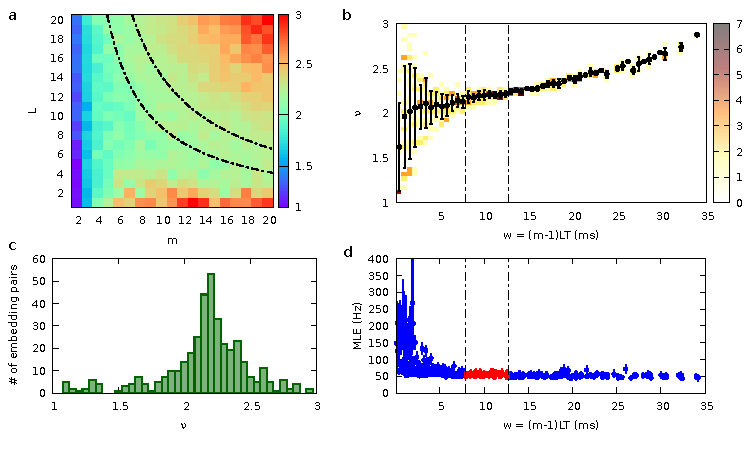
\includegraphics[width=\linewidth]{../2_blocks/1e5_points/plots/chaos.pdf}
    \caption{Edge}
    \label{fig:2 blocks chaos}
\end{figure}


\section{Three blocks}

\begin{figure}[H]
    \centering
    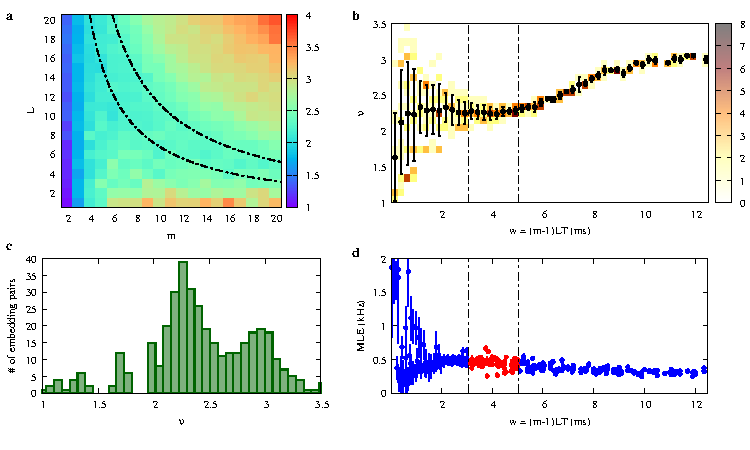
\includegraphics[width=\linewidth]{../3_blocks/edge/2e5_points/plots/chaos_low.pdf}
    \caption{Edge}
    \label{fig:3 blocks chaos}
\end{figure}

\section{Four blocks}

\begin{figure}[H]
    \centering
    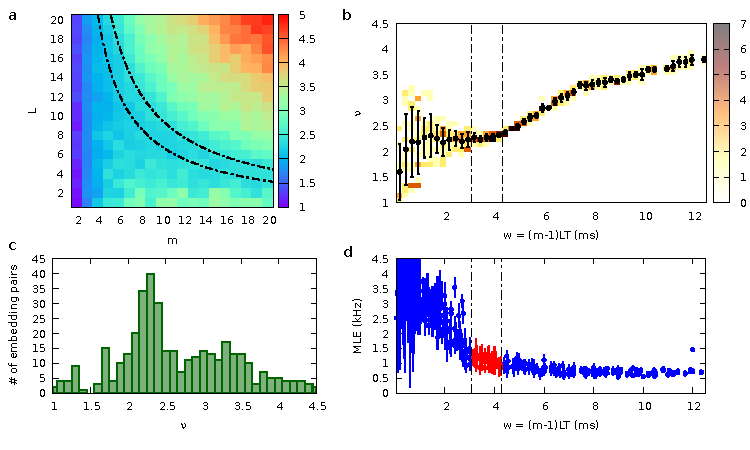
\includegraphics[width=\linewidth]{../4_blocks/2e5_points_new/plots/chaos_low.pdf}
    \caption{Edge}
    \label{fig:4 blocks chaos}
\end{figure}


\section{Five blocks}

\begin{figure}[H]
    \centering
    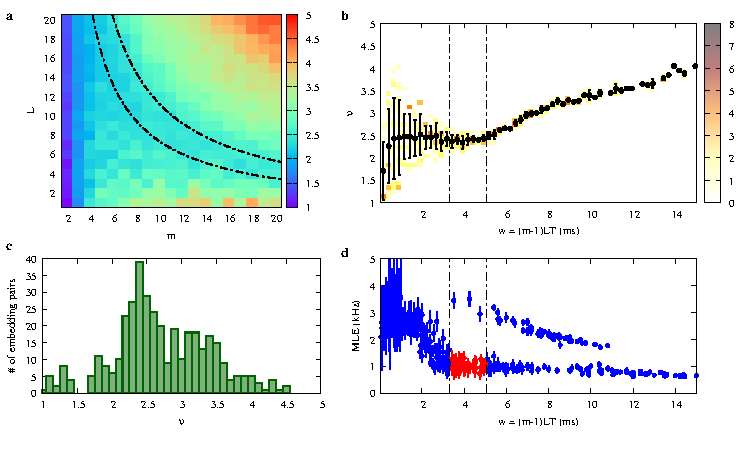
\includegraphics[width=\linewidth]{../5_blocks/edge/2e5_points/plots/chaos_low.pdf}
    \caption{Edge}
    \label{fig:5 blocks chaos}
\end{figure}

\section{Six blocks}

\begin{figure}[H]
    \centering
    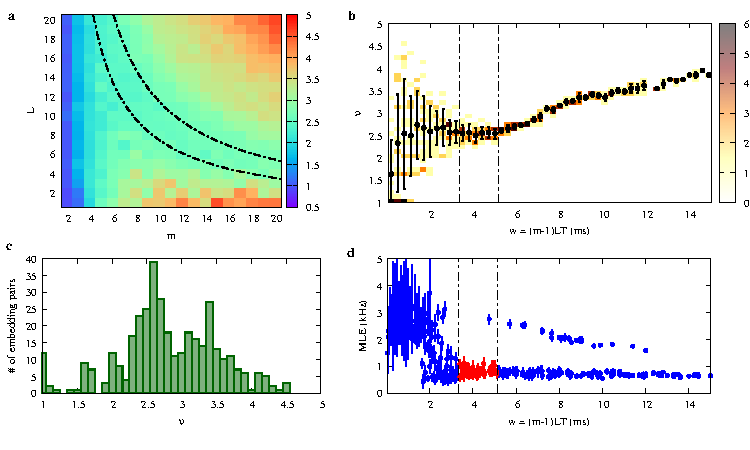
\includegraphics[width=\linewidth]{../6_blocks/2e5_points/plots/chaos_low.pdf}
    \caption{Edge}
    \label{fig:6 blocks chaos}
\end{figure}

\section{Seven blocks}

\begin{figure}[H]
    \centering
    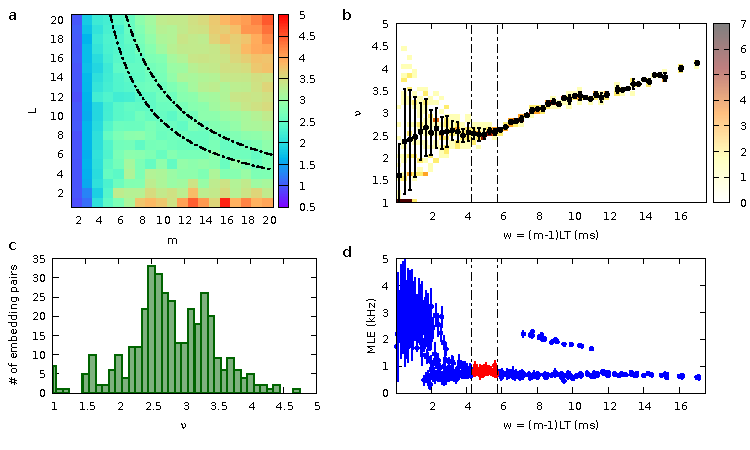
\includegraphics[width=\linewidth]{../7_blocks/edge/2e5_points/plots/chaos_low.pdf}
    \caption{Edge}
    \label{fig:7 blocks chaos}
\end{figure}

\section{Eight blocks}

\begin{figure}[H]
    \centering
    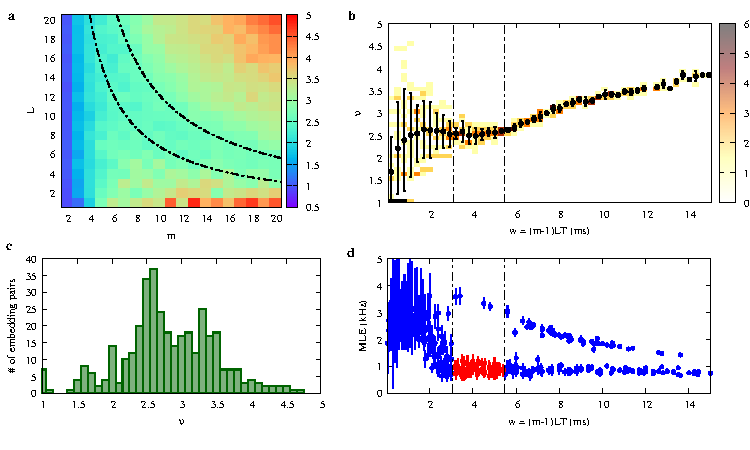
\includegraphics[width=\linewidth]{../8_blocks/2e5_points/plots/chaos_low.pdf}
    \caption{Edge}
    \label{fig:8 blocks chaos}
\end{figure}

\section{Nine blocks}

\begin{figure}[H]
    \centering
    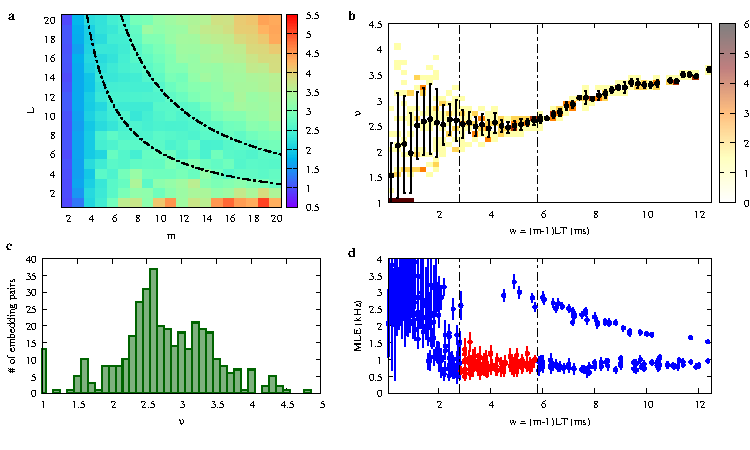
\includegraphics[width=\linewidth]{../9_blocks/edge/2e5_points/plots/chaos_low.pdf}
    \caption{Edge}
    \label{fig:9 blocks chaos}
\end{figure}

\begin{figure}[H]
    \centering
    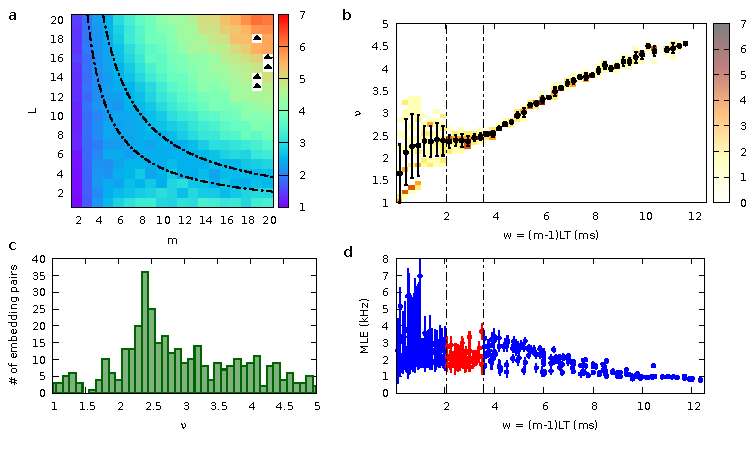
\includegraphics[width=\linewidth]{../9_blocks/middle/2e5_points/plots/chaos_low.pdf}
    \caption{Middle}
    \label{fig:9 blocks chaos middle}
\end{figure}

\section{Ten blocks}

\begin{figure}[H]
    \centering
    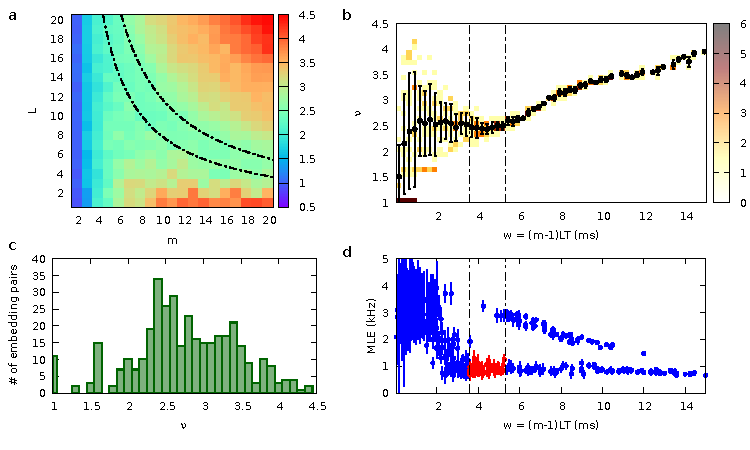
\includegraphics[width=\linewidth]{../10_blocks/2e5_points/plots/chaos_low.pdf}
    \caption{Edge}
    \label{fig:10 blocks chaos}
\end{figure}

\section{Conclusions}

\begin{figure}[H]
    \centering
    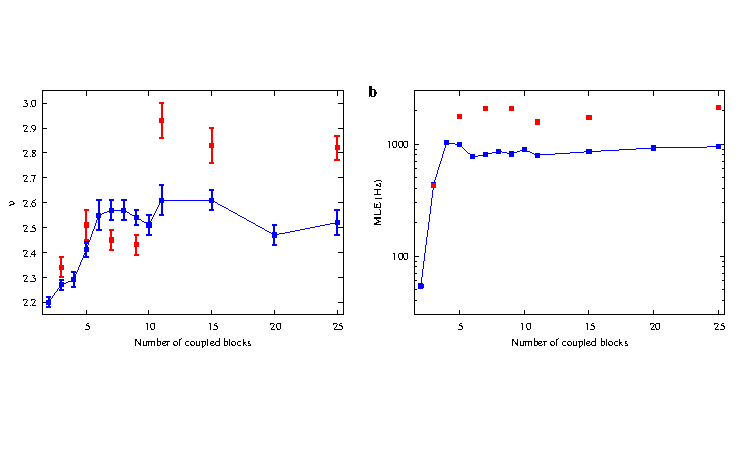
\includegraphics[width=\linewidth,trim={0 1.5cm 0 1.3cm},clip]
    {../data/nu_mle_blocks.pdf}
    \caption{Edge (blue) and middle (red)}
    \label{fig:nu mle blocks}
\end{figure}
